\documentclass[12pt,ngerman]{scrartcl}
\usepackage[T1]{fontenc}
\usepackage[latin9]{inputenc}
\setlength{\parskip}{\medskipamount}
\setlength{\parindent}{0pt}
\usepackage{float}
\usepackage{amsmath}
\usepackage{graphicx}

\makeatletter
\usepackage{babel}
\makeatother

\begin{document}

\part*{Trigonometrie}


\section{S�tze}


\subsection{Satz 1 bis 4}

$\cos(\alpha)=\cos(-\alpha)$

$\sin(90-\alpha)=\cos(\alpha)$

$\cos(90+\alpha)=-\sin(\alpha)$

$\sin(-\alpha)=-\sin(\alpha)$

\newpage{}


\subsection{Additionstheoreme (Reihenfolge=Beweise)}


\subsubsection{$\cos(\alpha-\beta)=\cos(\alpha)\cos(\beta)-\sin(\alpha)\sin(\beta)$}

%
\begin{figure}[H]
\caption{\protect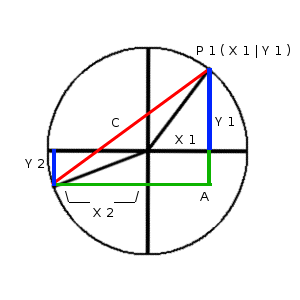
\includegraphics{beweis-cos-x-minus-y_graph-1}}

\end{figure}


$P_{1}AP_{2}\: rechtwinklig$

$P_{2}A=x_{1}-x_{2}$

$P_{1}A=y_{1}-y_{2}$

$c^{2}=(y_{1}-y_{2})^{2}+(x_{1}-x_{2})^{2}$

$c^{2}=y_{1}^{2}-2y_{1}y_{2}+y_{2}^{2}\;+\; x_{1}^{2}-2x_{1}x_{2}+x_{2}^{2}$

$c^{2}=x_{1}^{2}+y_{1}^{2}+x_{2}^{2}+y_{2}^{2}\;-\;2*(x_{1}x_{2}+y_{1}y_{2})$

$c^{2}=1+1\;-\;2*(x_{1}x_{2}+y_{1}y_{2})$

%
\begin{figure}[H]
\caption{\protect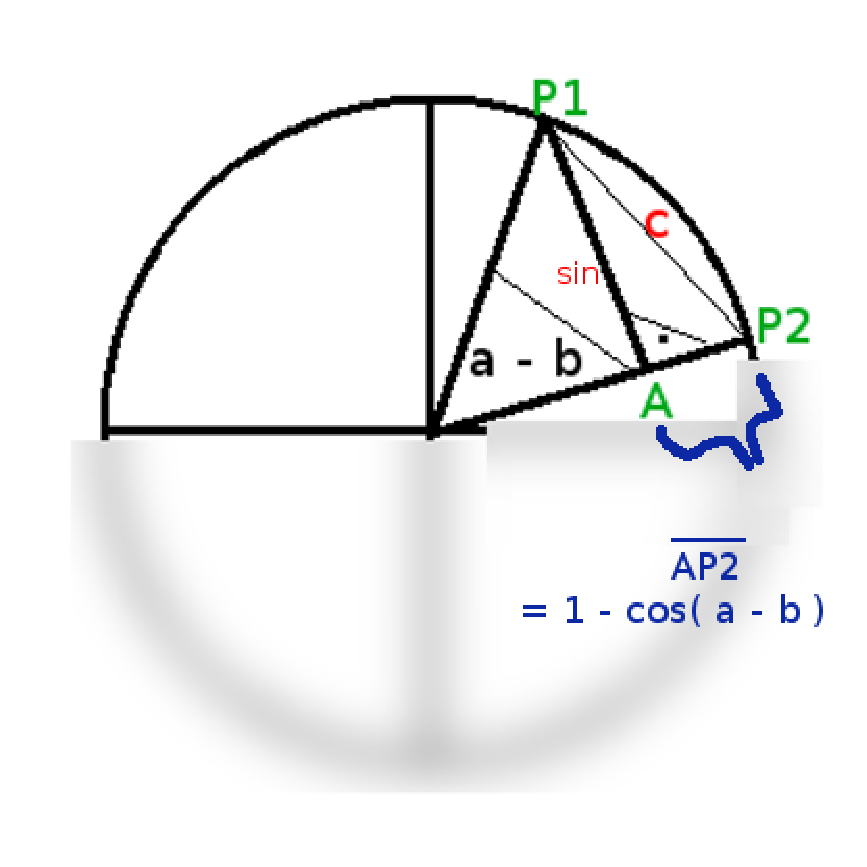
\includegraphics{beweis-cos-x-minus-y_graph-2}}

\end{figure}


$c^{2}=\overline{P_{1}A}^{2}+\overline{P_{2}A}^{2}$

Definition: $\varphi=\alpha-\beta$

$c^{2}=\sin^{2}(\varphi)+(1-\cos(\varphi))^{2}$

2. Binomische Formel: 

$c^{2}=\sin^{2}(\varphi)+1-2\cos(\varphi)+\cos^{2}(\varphi)$

$c^{2}=2-2\cos(\varphi)$

Ergebnis:

$c^{2}=2-2\cos(\alpha-\beta)=2-2(x_{1}x_{2}+y_{1}y_{2})$ | - 2 |
: (-2)

$c^{2}=\cos(\alpha-\beta)=x_{1}x_{2}+y_{1}y_{2}$

\clearpage{}


\subsubsection{$\cos(\alpha+\beta)=\cos(\alpha)*\cos(\beta)-\sin(\alpha)*\sin(\beta)$}

$\cos(\alpha+\beta)=\cos(\alpha-(-\beta))$\hfill{}>>+<< entspricht
>>- -<<

$\cos(\alpha+\beta)=\cos(\alpha)\cos(-\beta)+\sin(\alpha)\sin(-\beta)$\hfill{}Anwendung
von Satz aus 1.2.1

$\cos(\alpha+\beta)=\cos(\alpha)\cos(\beta)-\sin(\alpha)\sin(\beta)$\hfill{}Anwendung
von Satz 1 und 4


\subsubsection{$\sin(\alpha+\beta)=\cos(\alpha)*\sin(\beta)+\cos(\beta)*\sin(\alpha)$}

Satz 3:

$\cos(\varphi+90�)=-\sin(\varphi)$\hfill{}| {*} (-1)

$-\cos(\varphi+90�)=\sin(\varphi)$

\bigskip{}
$\varphi=\alpha+\beta$\hfill{}Definition (wegen �bersicht)

$\sin(\alpha+\beta)=-\cos(\alpha+\beta+90�)$

$\sin(\alpha+\beta)=-\cos(\alpha)\cos(\beta+90�)+\sin(\alpha)\sin(\beta+90�)$

$\sin(\alpha+\beta)=-\cos(\alpha)*-\sin(\beta)+\sin(\alpha)\cos(-\beta)$\hfill{}Anwendung
von Satz 2 und 3

$\sin(\alpha+\beta)=\cos(\alpha)\sin(\beta)+\sin(\alpha)\cos(\beta)$\hfill{}Anwendung
von Satz 1


\subsubsection{$\sin(\alpha-\beta)=\cos(\alpha)*\sin(\beta)-\cos(\beta)*\sin(\alpha)$}

$\sin(\alpha-\beta)=\sin(\alpha+(-\beta))$\hfill{}>>+<< entspricht
>>+ -<<

$\sin(\alpha+(-\beta))=\cos(-\beta)*\sin(\alpha)+\cos(\alpha)*\sin(-\beta)$\hfill{}

$\sin(\alpha+(-\beta))=\cos(\beta)\sin(\alpha)-\cos(\alpha)\sin(\beta)$\hfill{}Anwendung
Satz 1 und 4

\clearpage{}


\subsubsection{$\tan(\alpha+\beta)=\dfrac{\tan(\alpha)+\tan(\beta)}{1-\tan(\alpha)*\tan(\beta)}$}

$\tan(\alpha+\beta)=\dfrac{\sin(\alpha+\beta)}{\cos(\alpha+\beta)}$\hfill{}$\tan$
entspricht $\dfrac{\sin}{\cos}$

Anwendung der bisher bewiesenen S�tze:

$\tan(\alpha+\beta)=\dfrac{\cos(\alpha)*\sin(\beta)+\cos(\beta)*\sin(\alpha)}{\cos(\alpha)*\cos(\beta)-\sin(\alpha)*\sin(\beta)}$\hfill{}

Nun wird im Z�hler und im Nenner durch $\cos(\alpha)*\cos(\beta)$
dividiert, da in dem zu beweisenden Term im Nenner ein $1-$ steht.

$\tan(\alpha+\beta)=\dfrac{\dfrac{\cos(\alpha)*\sin(\beta)+\cos(\beta)*\sin(\alpha)}{\cos(\alpha)*\cos(\beta)}}{\dfrac{\cos(\alpha)*\cos(\beta)-\sin(\alpha)*\sin(\beta)}{\cos(\alpha)*\cos(\beta)}}$\hfill{}Division
im Z�hler und im Nenner

$\tan(\alpha+\beta)=\dfrac{\dfrac{\cos(\alpha)*\sin(\beta)}{\cos(\alpha)*\cos(\beta)}+\dfrac{\cos(\beta)*\sin(\alpha)}{\cos(\alpha)*\cos(\beta)}}{\dfrac{\cos(\alpha)*\cos(\beta)}{\cos(\alpha)*\cos(\beta)}-\dfrac{\sin(\alpha)*\sin(\beta)}{\cos(\alpha)*\cos(\beta)}}$\hfill{}

$\tan(\alpha+\beta)=\dfrac{\dfrac{\sin(\beta)}{\cos(\beta)}+\dfrac{\sin(\alpha)}{\cos(\alpha)}}{1-\dfrac{\sin(\alpha)*\sin(\beta)}{\cos(\alpha)*\cos(\beta)}}$\hfill{}K�rzen

$\tan(\alpha+\beta)=\dfrac{\tan(\beta)+\tan(\alpha)}{1-\tan(\beta)*\tan(\alpha)}$\hfill{}$\dfrac{\sin}{\cos}$
entspricht $\tan$

\clearpage{}


\subsubsection{$\tan(\alpha-\beta)=\dfrac{\tan(\alpha)+\tan(\beta)}{1+\tan(\alpha)*\tan(\beta)}$}

$\tan(\alpha-\beta)=\dfrac{\sin(\alpha-\beta)}{\cos(\alpha-\beta)}$\hfill{}$\tan$
entspricht $\dfrac{\sin}{\cos}$

Anwendung der bisher bewiesenen S�tze:

$\tan(\alpha-\beta)=\dfrac{\cos(\alpha)*\sin(\beta)-\cos(\beta)*\sin(\alpha)}{\cos(\alpha)*\cos(\beta)+\sin(\alpha)*\sin(\beta)}$\hfill{}

Nun wird im Z�hler und im Nenner durch $\cos(\alpha)*\cos(\beta)$
dividiert, da in dem zu beweisenden Term im Nenner ein $1+$ steht.

$\tan(\alpha-\beta)=\dfrac{\dfrac{\cos(\alpha)*\sin(\beta)-\cos(\beta)*\sin(\alpha)}{\cos(\alpha)*\cos(\beta)}}{\dfrac{\cos(\alpha)*\cos(\beta)+\sin(\alpha)*\sin(\beta)}{\cos(\alpha)*\cos(\beta)}}$\hfill{}Division
im Z�hler und im Nenner

$\tan(\alpha-\beta)=\dfrac{\dfrac{\cos(\alpha)*\sin(\beta)}{\cos(\alpha)*\cos(\beta)}-\dfrac{\cos(\beta)*\sin(\alpha)}{\cos(\alpha)*\cos(\beta)}}{\dfrac{\cos(\alpha)*\cos(\beta)}{\cos(\alpha)*\cos(\beta)}+\dfrac{\sin(\alpha)*\sin(\beta)}{\cos(\alpha)*\cos(\beta)}}$\hfill{}

$\tan(\alpha-\beta)=\dfrac{\dfrac{\sin(\beta)}{\cos(\beta)}-\dfrac{\sin(\alpha)}{\cos(\alpha)}}{1+\dfrac{\sin(\alpha)*\sin(\beta)}{\cos(\alpha)*\cos(\beta)}}$\hfill{}K�rzen

$\tan(\alpha-\beta)=\dfrac{\tan(\beta)+\tan(\alpha)}{1+\tan(\beta)*\tan(\alpha)}$\hfill{}$\dfrac{\sin}{\cos}$
entspricht $\tan$

\clearpage{}


\subsubsection{$\cot(\alpha+\beta)=\dfrac{\cot(\alpha)*\cot(\beta)-1}{\cot(\beta)-\cot(\alpha)}$}

$\cot(\alpha+\beta)=\dfrac{\cos(\alpha+\beta)}{\sin(\alpha+\beta)}$\hfill{}$\cot$
entspricht $\dfrac{\cos}{\sin}$

Anwendung der bisher bewiesenen S�tze:

$\cot(\alpha+\beta)=\dfrac{\cos(\alpha)*\cos(\beta)-\sin(\alpha)*\sin(\beta)}{\cos(\alpha)*\sin(\beta)+\cos(\beta)*\sin(\alpha)}$\hfill{}

Nun wird im Z�hler und im Nenner durch $\sin(\alpha)*\sin(\beta)$
dividiert, da in dem zu beweisenden Term im Z�hler ein $-1$ steht.

$\cot(\alpha+\beta)=\dfrac{\dfrac{\cos(\alpha)*\cos(\beta)-\sin(\alpha)*\sin(\beta)}{\sin(\alpha)*\sin(\beta)}}{\dfrac{\cos(\alpha)*\sin(\beta)+\cos(\beta)*\sin(\alpha)}{\sin(\alpha)*\sin(\beta)}}$\hfill{}Division
im Z�hler und im Nenner

$\cot(\alpha+\beta)=\dfrac{\dfrac{\cos(\alpha)*\cos(\beta)}{\sin(\alpha)*\sin(\beta)}-\dfrac{\sin(\alpha)*\sin(\beta)}{\sin(\alpha)*\sin(\beta)}}{\dfrac{\cos(\alpha)*\sin(\beta)}{\sin(\alpha)*\sin(\beta)}+\dfrac{\cos(\beta)*\sin(\alpha)}{\sin(\alpha)*\sin(\beta)}}$\hfill{}

$\cot(\alpha+\beta)=\dfrac{\cot(\alpha)*\cot(\beta)-1}{\cot(\alpha)+\cot(\beta)}$\hfill{}K�rzen

\clearpage{}


\subsubsection{$\cot(\alpha-\beta)=\dfrac{\cot(\alpha)*\cot(\beta)+1}{\cot(\beta)-\cot(\alpha)}$}

$\cot(\alpha-\beta)=\dfrac{\cos(\alpha-\beta)}{\sin(\alpha-\beta)}$\hfill{}$\cot$
entspricht $\dfrac{\cos}{\sin}$

Anwendung der bisher bewiesenen S�tze:

$\cot(\alpha-\beta)=\dfrac{\cos(\alpha)*\cos(\beta)+\sin(\alpha)*\sin(\beta)}{\cos(\alpha)*\sin(\beta)-\cos(\beta)*\sin(\alpha)}$\hfill{}

Nun wird im Z�hler und im Nenner durch $\sin(\alpha)*\sin(\beta)$
dividiert, da in dem zu beweisenden Term im Z�hler ein $+1$ steht.

$\cot(\alpha-\beta)=\dfrac{\dfrac{\cos(\alpha)*\cos(\beta)+\sin(\alpha)*\sin(\beta)}{\sin(\alpha)*\sin(\beta)}}{\dfrac{\cos(\alpha)*\sin(\beta)-\cos(\beta)*\sin(\alpha)}{\sin(\alpha)*\sin(\beta)}}$\hfill{}Division
im Z�hler und im Nenner

$\cot(\alpha-\beta)=\dfrac{\dfrac{\cos(\alpha)*\cos(\beta)}{\sin(\alpha)*\sin(\beta)}+\dfrac{\sin(\alpha)*\sin(\beta)}{\sin(\alpha)*\sin(\beta)}}{\dfrac{\cos(\alpha)*\sin(\beta)}{\sin(\alpha)*\sin(\beta)}-\dfrac{\cos(\beta)*\sin(\alpha)}{\sin(\alpha)*\sin(\beta)}}$\hfill{}

$\cot(\alpha-\beta)=\dfrac{\cot(\alpha)*\cot(\beta)+1}{\cot(\alpha)-\cot(\beta)}$\hfill{}K�rzen

\clearpage{}


\subsubsection{$\sin(2\alpha)=2\sin(\alpha)\cos(\alpha)$}

$\sin(2\alpha)=\sin(\alpha+\alpha)=\sin(\alpha)\cos(\alpha)+\cos(\alpha)\sin(\alpha)$

$\sin(2\alpha)=2*\sin(\alpha)\cos(\alpha)$


\subsubsection{$\cos(2\alpha)=1-2\sin^{2}(\alpha)$}

$\cos(2\alpha)=\cos(\alpha+\alpha)=\cos(\alpha)\cos(\alpha)-\sin(\alpha)\sin(\alpha)$

$\cos(2\alpha)=\cos^{2}(\alpha)-\sin^{2}(\alpha)$

Addition von: $+\sin^{2}(\alpha)-\sin^{2}(\alpha)=0$

$\cos(2\alpha)=\cos^{2}(\alpha)-\sin^{2}(\alpha)+\sin^{2}(\alpha)-\sin^{2}(\alpha)$

$\rightarrow$$\cos^{2}(\alpha)-\sin^{2}(\alpha)+\sin^{2}(\alpha)=1$

$\Rightarrow$$\cos(2\alpha)=1-2\sin^{2}(\alpha)$


\subsubsection{$\left|\sin\dfrac{\alpha}{2}\right|=\sqrt{\dfrac{1-\cos(\alpha)}{2}}$}

Gegeben: $\cos(2\alpha)=1-2\sin^{2}(\alpha)$

$\alpha=2*\dfrac{\alpha}{2}$

$\cos(2\dfrac{\alpha}{2})=1-2\sin^{2}(\dfrac{\alpha}{2})$

$\cos(\alpha)=1-2\sin^{2}(\dfrac{\alpha}{2})$\hfill{}|$-1$

$\cos(\alpha)-1=-2\sin^{2}(\dfrac{\alpha}{2})$\hfill{}|$/(-2)$

$\dfrac{\cos(\alpha)-1}{-2}=\sin^{2}(\dfrac{\alpha}{2})$\hfill{}Umformen

$\dfrac{1-\cos(\alpha)}{2}=\sin^{2}(\dfrac{\alpha}{2})$\hfill{}|Quadratwurzel

$\sqrt{\dfrac{1-\cos(\alpha)}{2}}=\left|\sin(\dfrac{\alpha}{2})\right|$\hfill{}|Quadratwurzel

\clearpage{}


\subsubsection{$\left|\cos\dfrac{\alpha}{2}\right|=\sqrt{\dfrac{1+\cos(\alpha)}{2}}$}

Gegeben: $\cos(2\alpha)=1-2\sin^{2}(\alpha)$

$\alpha=2*\dfrac{\alpha}{2}$

$\cos(2\dfrac{\alpha}{2})=1-2\sin^{2}(\dfrac{\alpha}{2})$

\medskip{}


Ersetzen der >>1<<, weil:

\[
1=\cos^{2}(\beta)+\sin^{2}(\beta)\]


$\cos(\alpha)=\cos^{2}(\beta)+\sin^{2}(\beta)-2\sin^{2}(\dfrac{\alpha}{2})$\hfill{}

$\cos(\alpha)=\cos^{2}(\beta)-\sin^{2}(\dfrac{\alpha}{2})$\hfill{}Weil:
$x-2x=-x$

Anwendung der zuletzt bewiesenen Formel:

\[
\cos(\alpha)=\cos^{2}(\beta)-\dfrac{1-\cos(\alpha)}{2}\]
\hfill{}

Quadrat alleine rechts, weil im zu beweisenden Term eine Quadratwurzel
vorkommt:

\[
\cos(\alpha)+\dfrac{1-\cos(\alpha)}{2}=\cos^{2}(\beta)\]
\hfill{}

Gleicher Nenner:

\[
\dfrac{2\cos(\alpha)+1-\cos(\alpha)}{2}=\cos^{2}(\beta)\]
\hfill{}

Zusammenfassen:

\[
\dfrac{1+\cos(\alpha)}{2}=\cos^{2}(\beta)\]
\hfill{}

Wurzel ziehen:

\[
\sqrt{\dfrac{1+\cos(\alpha)}{2}}=\cos(\beta)\]
\hfill{}

\clearpage{}


\subsubsection{$\sin(3\alpha)=3\sin(\alpha)-4\sin^{3}(\alpha)$}

$\sin(3\alpha)=\sin(2\alpha+\alpha)$

\[
=\cos(2\alpha)\sin(\alpha)+\cos(\alpha)\sin(2\alpha)\]


Vertauschen, kommutativ:

\[
=\cos(\alpha)\sin(2\alpha)+\cos(2\alpha)\sin(\alpha)\]


Anwendung der letzten beiden Formeln:

\[
=\cos(\alpha)*[2\sin(\alpha)\cos(\alpha)]+\sin(\alpha)*[1-2\sin^{2}(\alpha)]\]


Umformen:

\[
=2\sin(\alpha)\cos^{2}(\alpha)+\sin(\alpha)-2\sin^{3}(\alpha)\]


Ausklammern: (Hintergrund: Es darf kein >>$\cos$<< vorkommen, n�chster
Schritt...)

\[
=2\sin(\alpha)\:*\:[\:\cos^{2}(\alpha)\:-\:\sin^{2}(\alpha)\:]\:+\sin(\alpha)\]


Anwenden: $-y=y-2y$

\[
=2\sin(\alpha)\:*\:[\:\cos^{2}(\alpha)\:+\:\sin^{2}(\alpha)\:-\:2\sin^{2}(\alpha)\:]\:+\sin(\alpha)\]


Anwenden: $1=\cos^{2}(\beta)+\sin^{2}(\beta)$

\[
=2\sin(\alpha)\:*\:[\:1\:-\:2\sin^{2}(\alpha)\:]\:+\sin(\alpha)\]


\[
=2\sin(\alpha)*1\:-\:4\sin^{3}(\alpha)\:+\sin(\alpha)\]


\[
=3\sin(\alpha)*1\:-\:4\sin^{3}(\alpha)\]

\end{document}
